\documentclass{beamer}
\usepackage[utf8]{inputenc}
\usepackage[brazil]{babel}
\usepackage{graphicx}

\usetheme{Berkeley}
\usecolortheme{crane}

\title{Apresentação \LaTeX}

\author{
    Victor Santos Nunes \inst{1}
    \and 
    Fulano de Tal \inst{2}
}

\institute{
    \inst{1} Departamento de Física\\Universidade Federal de Sergipe
    \and
    \inst{2} Coordenadoria de Engenharia\\Universidade Tiradentes
}

\date{August 2021}

\begin{document}

\frame{\titlepage} %É equivalente ao \maketitle

\begin{frame}{Sumário}
    \tableofcontents
\end{frame}

\begin{frame}
    \frametitle{Disclaimer}
    Lorem ipsum dolor sit amet, consectetur adipiscing elit. Morbi aliquet nulla vitae lacus congue aliquam. Nulla luctus orci vel fermentum vehicula. Phasellus at gravida nisi. Etiam porttitor rhoncus elit in ultricies. Vestibulum mollis odio id massa cursus fermentum. Nam efficitur, leo vel bibendum malesuada, nibh felis lacinia tortor, quis efficitur ligula sem id ex. Proin ex est, blandit eu vestibulum nec, imperdiet quis mauris.
\end{frame}

\begin{frame}{Exemplo 1}
    \section{Exemplo 1}
    Lorem ipsum dolor sit amet, consectetur adipiscing elit. Morbi aliquet nulla vitae lacus congue aliquam. Nulla luctus orci vel fermentum vehicula. Phasellus at gravida nisi. Etiam porttitor rhoncus elit in ultricies. Vestibulum mollis odio id massa cursus fermentum. Nam efficitur, leo vel bibendum malesuada, nibh felis lacinia tortor, quis efficitur ligula sem id ex. Proin ex est, blandit eu vestibulum nec, imperdiet quis mauris.
\end{frame}

\begin{frame}{Lista}
    \section{Lista}
    \begin{itemize}
        \item Item 1
        \item Item 2
        \item Item 3
        \item Item 4
    \end{itemize}
\end{frame}

\begin{frame}{Lista com "Animação"}
\section{Lista com Animação}
    \begin{itemize}
        \item<1-> Item 1
        \item<2-> Item 2
        \item<3-> Item 3
        \item<4-> Item 4
    \end{itemize}
\end{frame}

\begin{frame}{Blocos}
    \section{Blocos}
    \begin{block}{Teorema da Alfândega}
        Lorem ipsum dolor sit amet, consectetur adipiscing elit. Morbi aliquet nulla vitae lacus congue aliquam. Nulla luctus orci vel fermentum vehicula. Phasellus at gravida nisi. Etiam porttitor rhoncus elit in ultricies. 
    \end{block}
    \begin{exampleblock}{Teorema de Stokes}
        Lorem ipsum dolor sit amet, consectetur adipiscing elit. Morbi aliquet nulla vitae lacus congue aliquam. Nulla luctus orci vel fermentum vehicula. Phasellus at gravida nisi. Etiam porttitor rhoncus elit in ultricies. 
    \end{exampleblock}
    \begin{alertblock}{Alert Block}
     Phasellus at gravida nisi. Etiam porttitor rhoncus elit in ultricies. 
    \end{alertblock}
\end{frame}

\begin{frame}{Colunas}
    \section{Colunas}
    \begin{columns}
        \column{0.5\textwidth}
        $$F = M \ a$$
        \begin{itemize}
            \item F = força
            \item M = massa
            \item a = aceleração
        \end{itemize}
        
        \column{0.5\textwidth}
        Lorem ipsum dolor sit amet, consectetur adipiscing elit. Morbi aliquet nulla vitae lacus congue aliquam. Nulla luctus orci vel fermentum vehicula. Phasellus at gravida nisi.
        
    \end{columns}
\end{frame} 

{
\usebackgroundtemplate{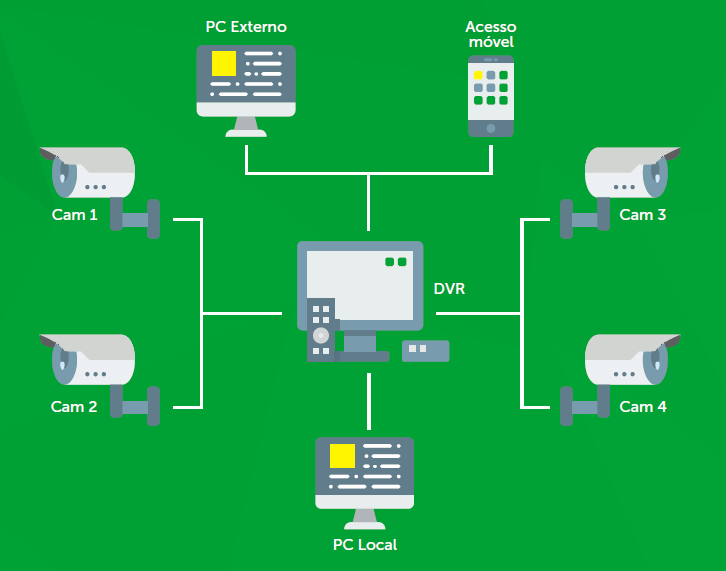
\includegraphics[scale=0.8]{equipamentos-de-cftv.png}}
\begin{frame}{Imagem de Fundo}
    \section{Imagem de Fundo}
    \color{red} \textbf{Lorem ipsum dolor sit amet, consectetur adipiscing elit. Morbi aliquet nulla vitae lacus congue aliquam. Nulla luctus orci vel fermentum vehicula. Phasellus at gravida nisi.}
\end{frame}
}

{
\setbeamertemplate{background canvas}[vertical shading][bottom=blue, top=white]
\begin{frame}{Fundo Gradiente}
\section{Fundo Gradiente}
    
\end{frame}
}

{
\setbeamercolor{normal text}{bg=green}
\begin{frame}{Cor Sólida}
    \section{Cor Sólida}
\end{frame}
}

\begin{frame}{Misturando as Coisas}
    \section{Misturando as Coisas}
    \begin{minipage}{0.58\textwidth}
        \begin{figure}
            \centering
            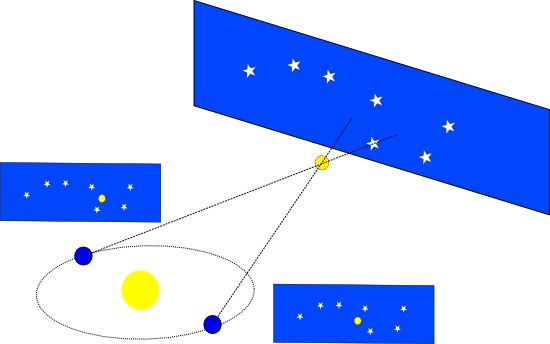
\includegraphics[scale=0.25]{ParallaxeV2.png}
            \caption{Paralaxe}
            \label{fig:my_label}
        \end{figure}
    \end{minipage}
    \hfill
    \begin{minipage}{0.36\textwidth}
        \begin{block}{Teorema}
        \centering
            $\sigma \left(\sum_i w_i x_1 + b \right)$
        \end{block}
        
        \begin{exampleblock}{Corolário}
            \centering
            $L_i = -log(\frac{e^{f_{y_i}}}{\sum_j e^{f_j}})$\\[0.1cm]
            cross entropy
        \end{exampleblock}
    \end{minipage}
\end{frame}

\end{document}
